\documentclass[output=paper,colorlinks,citecolor=brown
% ,hidelinks
% showindex
]{langscibook}

\title[Contextualizing typologically remarkable sound patterns in Pirahã]{Contextualizing typologically remarkable sound patterns in Pirahã: A quantitative approach}
\abstract{The sound system of Pirahã includes several remarkable phenomena. The present work seeks to illuminate some of those phenomena via the typological contextualization of a few of the most unusual phonetic and phonological features of the language. The study relies on previous research as well as new analyses of transcribed word lists in the UCLA Phonetics Lab Archive, alongside analyses of crosslinguistic databases of phoneme inventories and word lists. Three phenomena are focused upon: i) The small phoneme inventory in the language, contextualized against the distribution of phoneme inventories worldwide. ii) The vowel formant space of adult Pirahã speakers. iii) The unusually high reliance on vowels and glottal consonants, and the concomitant rarity of oral consonants and consonant clusters in this Amazonian isolate. This latter suite of interrelated features is uncovered via contrasts of patterns in Pirahã word lists with those of over four thousand language varieties worldwide. The language’s high degree of reliance on vowels and glottal consonants is perhaps the most remarkable feature of its sound system, given that it is a statistical outlier in this respect. I suggest that this unusual feature may contribute to the challenges outsiders face when trying to learn the language.}
\author{Caleb Everett}

\begin{document}
\label{chap-13_everett}

\maketitle

\section{Background}

Pirahã is an Amazonian isolate with a number of typologically unusual characteristics. Daniel
Everett, my father, brought attention to this language through a series of studies published over
the last few decades, based on his extensive fieldwork \citep{everett1982phonetic,
  everett1984relevance,everett1986piraha,everett2001monolingual}. These studies include evidence for
the language's lack of number words, which has been verified experimentally by other scholars
\citep{frank2008number, everett2012quantity}. The language also exhibits rarities in other lexical
domains, including its terms for colors and kin relationships \citep{everett2005cultural}. It displays uncommon morphological and syntactic characteristics as well \citep{thomason2001pronoun, everett2012language}. Most famously, there is an absence of evidence for syntactic recursion in the language \citep{everett2005cultural}. A study of a corpus of transcribed clauses supports this absence, to the extent that it yielded no evidence that Pirahã grammar allows recursive clauses \citep{futrell2016corpus}. While such lexical and morphosyntactic characteristics are certainly rare crosslinguistically, some of them are apparently found in other languages. Absence of recursion has been claimed for several languages, for instance, and other languages lack, or once lacked, precise number words \citep{pullum2020theorizing, everett2017numbers}.
    
    \begin{sloppypar}
    The phonetic and phonological characteristics of Pirahã are also unusual in some regards. For instance, the language has one of the world’s smallest phoneme inventories \citep{everett2009piraha}. It also exhibits unusual socio-phonetic variation across genders: Women can produce a voiceless alveolar fricative instead of a voiceless glottal fricative, though this sociolinguistic variation may be more pronounced in some villages. (Keren Madora, personal communication) Another intriguing feature is the presence of onset-sensitive stress, which was not attested crosslinguistically prior to the publication of \citew{everett1984relevance}. Also, the language has one very unusual allophone, a flap that requires tongue contact at both the alveolar ridge and the lower lip, and in so doing requires tongue protrusion from the mouth \citep{everett1982phonetic}.
    \end{sloppypar}
    
    Many of Pirahã’s remarkable characteristics owe themselves at least partially to its status as a language isolate, the last survivor of the Mura family. Another factor involved in promoting these unusual characteristics is the culture of the people, which proscribes the adoption of most aspects of other cultures, including number words \citep{everett2005cultural}. In the next two sections I offer some discussion of a few of the typologically remarkable phonetic and phonological features of the language, though this is not meant to be an exhaustive review of those features, especially since many of these features have been documented extensively in the literature -- largely through the work of my father. In section 2 we will examine the language’s small phoneme inventory, contextualizing it against patterns evident in worldwide surveys of phoneme inventories. In section 3 we will examine some of the language’s phonotactic features, demonstrating with a novel approach that the language is quite unusual in terms of its reliance on vowels and glottal consonants. I suggest that the latter feature likely contributes to the well-known difficulty of non-Pirahã acquiring the language, which has been observed for the last several decades. In section 4 I offer some concluding remarks. 


\section{The phoneme inventory}

    The Pirahã phoneme inventory is famously quite small, with eight consonants and three vowels, though the figure of eight consonants is open to some debate given the socio-phonetic variation mentioned above for the alveolar and glottal fricative. However, the phoneme inventory is relatively normal in terms of its phoneme types. The four voiceless stops in the language are /p/, /t/, /k/, and /{\textglotstop}/. The first three of these voiceless stops are among the most common phonemes, in terms of both crosslinguistic frequency and frequency within word lists across about 7000 word lists and over 3000 phoneme inventories \citep{everett2018similar, everett2021sounds}. The two voiced stops are /b/, which has an [m] allophone, and /g/, which has an [n] allophone. The language is somewhat unusual in that it is missing a voiced alveolar plosive phoneme but has a voiced velar plosive. The reverse pattern is much more common typologically \citep{everett2018global}. As noted above, there is also a glottal fricative with an alveolar fricative variant in the language \citep{everett1986piraha}. All of these consonants are quite common crosslinguistically. Similarly, while Pirahã only has three vowel phonemes, these are peripheral vowels with very distinct formant characteristics, vowels we might expect in a three-vowel system: /a/, /i/ and /o/.

    To get a sense of how common these consonants and vowels are crosslinguistically, we can look at the PHOIBLE database of 3,183 phoneme inventories \citep{phoible}. There we see that /k/ is found in over 90\% of the world’s languages, and is the most common voiceless stop typologically. /p/ is found in about 86\% of the world’s languages, while /t/ is found in 68\% of them. /b/ and /g/ are found in 63\% and 57\% of the world’s languages, respectively. /h/ is found in 56\% of PHOIBLE inventories. Turning to the vowels, /i/ and /a/ are found in 92\% and 86\% of the world’s phoneme inventories, respectively, while /o/ is found in 60\%. The only phoneme in Pirahã that is not found in well over half of the world’s languages is the glottal stop, and even that sound is fairly common as a phoneme, as it is found in 37\% of the phoneme inventories in PHOIBLE.

    While the language has one of the world’s smallest phoneme inventories, then, most its phonemes are quite common typologically. Also, it is worth noting that many of the world's phoneme inventories are not much larger than that of Pirahã. Framed differently, if we plot a density distribution based on the number of phonemes in the world’s phoneme inventories, the values representing phoneme inventory size will be compressed along the leftmost portion of the x-axis. The same can be said if we plot the number of consonant phonemes or vowel phonemes. This is evident in Figure 1, which includes three density distributions of phoneme-inventory sizes, based on the UCLA phonological segments inventory database (USPID) \citep{maddieson1989updating}. That database contains 451 phoneme inventories from around the world.
        
    \begin{figure}
    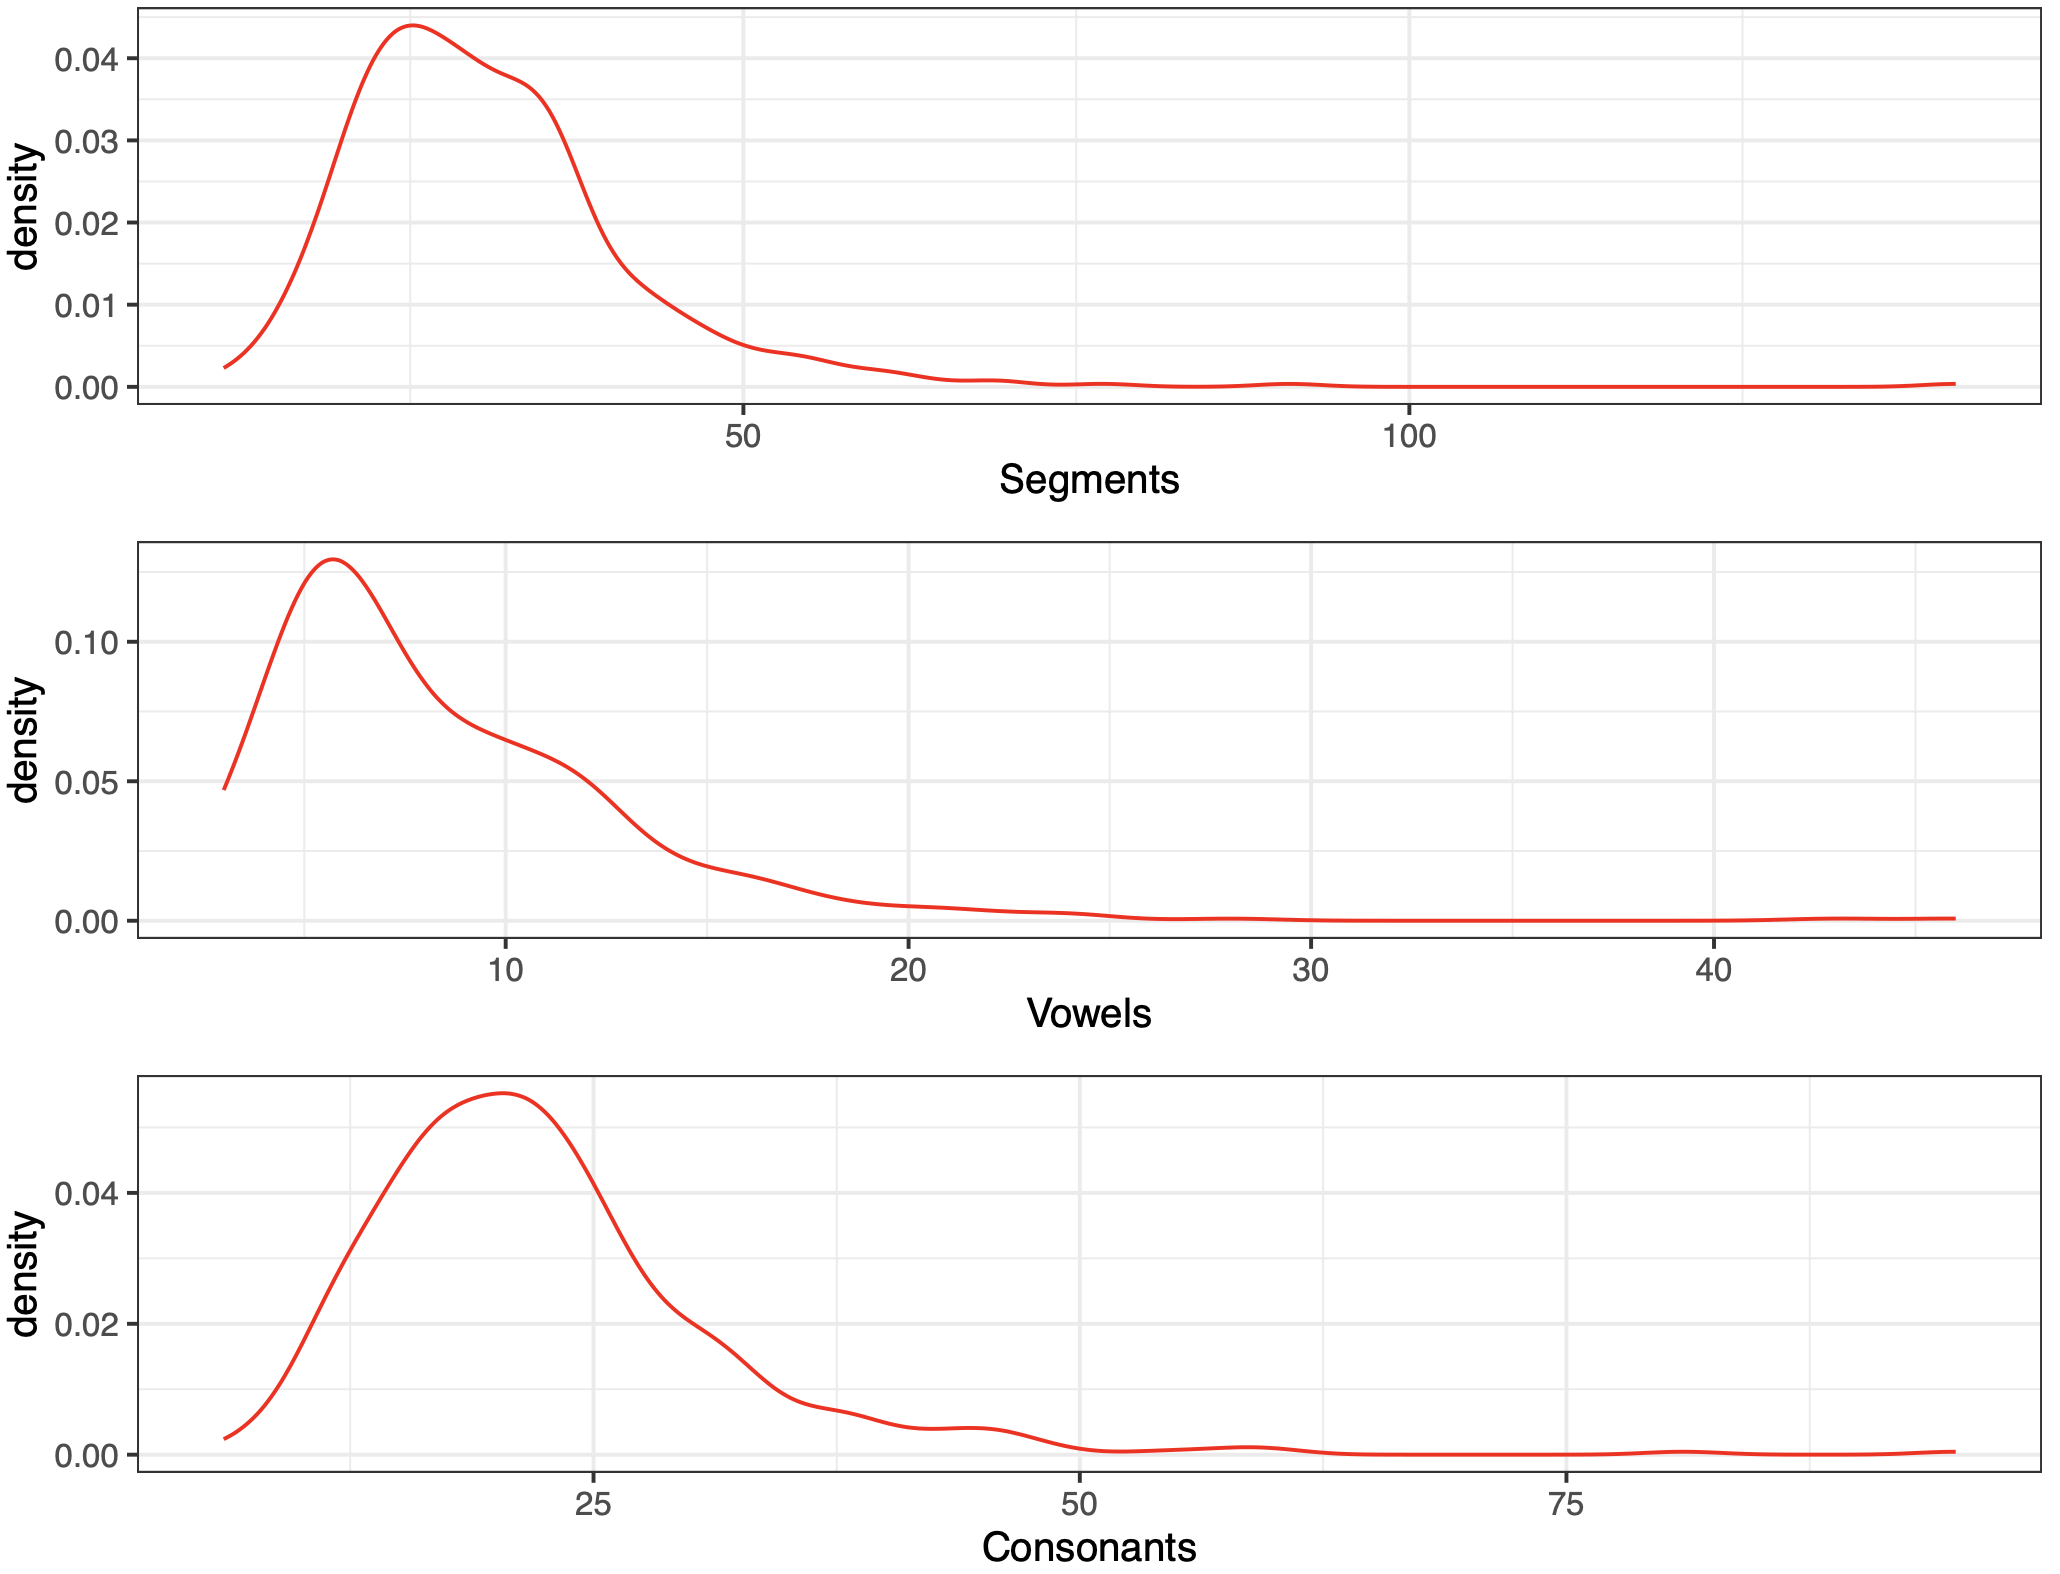
\includegraphics[width=\textwidth]{figures/everett_figure1.png}
    \caption{\label{fig:Figure 1}Density distributions of the number of phonemic segments, vowels, and consonants across the world’s phoneme inventories. This is based on 451 languages in the UPSID database \citep{maddieson1989updating}.}
    \end{figure}

    As is evident in Figure 1, the world’s phoneme inventories range dramatically in size, but the vast majority have fewer than fifty total phonemic segments. The typological outliers are those languages at the far-right end of the distribution of phoneme, vowel and consonant inventories. Languages like Danish, with dozens of vowel phonemes, and Xóõ, with over ninety consonants according to UPSID (estimates vary), are such outliers. If we take a common approach to defining outliers, an upper-limit outlier would include any language with a phoneme inventory that is above the third quartile by greater than 1.5 times the IQR (interquartile range). Under this approach, a phoneme inventory in UPSID would need to exceed 55 phonemes to be an outlier. There are seven phoneme inventories in the data set that do exceed this figure. Conversely, a lower-limit outlier would include any language with a phoneme inventory that is below the first quartile by 1.5 times the IQR. A phoneme inventory in UPSID would need to have fewer than five phonemes to be an outlier in this respect. Of course, no languages exhibit such a small phoneme inventory. The truth is that many languages have small sets of vowel and/or consonant phonemes, so there are no outliers on this end of the phoneme-inventory spectrum. Framed differently, many languages have one-to-a-few more phonemes than Pirahã. This pattern is apparent not just in these data but in large studies on phonological typology, for instance \citew{gordon2016phonological}. Nevertheless, Pirahã is certainly unusual in that it is small both in terms of its consonant inventory and vowel inventory -- setting aside that it does use tones, in contrast to some other languages with three vowel phonemes. In the UPSID data, 23 of 451 languages have inventories with three vowels and many of these are not tonal. In contrast, only five of the 451 languages in that database have eight or fewer consonant phonemes. 
    
    Pirahã also has straightforward syllable structure. If we examine the 150 words representing Pirahã in the UCLA Phonetics Lab Archive, we see that all of the words contain syllables of either the CV or CVV type, and only these two types of syllable are represented. Both of these syllable types are common worldwide. In Maddieson’s survey of the syllable structure types in 486 languages, 61 languages are categorized as having simple syllable types \citep{wals12}. Pirahã would fall into this category, which is not a particularly rare one. While Pirahã has simple syllable structure along with a small phoneme inventory that consists of a straightforward set of common vowels and consonants, these points do not imply that the language is simple, overall, in terms of its phonological or phonetic characteristics. To the contrary, there is arguably unusual complexity in the language’s sound system, at least from the perspective of learners of the language, a point I will aim to quantify below. This complexity stems from the fact that the language is tonal and relies heavily on vowels, yielding words that are distinguished inordinately by vocalic characteristics without many intervening oral consonants. This is one factor contributing to the fact that the acquisition of the language is notoriously difficult, particularly for speakers of English and Portuguese who lack familiarity with tones and are unable to easily distinguish the distinct tones of adjacent vowels. This point, to which I will return in the conclusion, is based on my own experience with the language, having seen many outsiders struggle to distinguish or reproduce Pirahã words. It is also based on the simple fact that, to date, few outside speakers have learned Pirahã well, arguably only two in fact: Dan Everett and Keren Madora.  
    
    Previous acoustic studies of Pirahã vowels have described the formant space in the language. Keren Madora, in a description of stress correlates in the language, describes the mean formant space for the /a/ and /i/ vowels across twelve adult speakers \citep{everett1998acoustic}. These are evident in Figure 2. \citet{de2010vowel} describes the formant space of the three vowels for two male adult speakers and one female. Carvalho also relied on the Pirahã data in the UCLA Phonetics Lab Archive. These data were collected by Peter Ladefoged, with the assistance of Dan Everett and Keren Madora, in 1995. The mean formant values for these three speakers are also depicted in the formant space depicted in Figure 1. Note that the /a/ vowel is articulated at a wide range of points along the F1 dimension, suggesting some freedom in tongue height for this vowel. In contrast, the /i/ and /o/ vowels appear to occur in a more constricted portion of the vowel space. An important caveat is that, since these formant values are not normalized, they do not necessarily reflect meaningful inter-speaker variation. Formant values are affected by vocal-tract length, for instance, which varies across speakers. It is not particularly surprising that the lone female speaker, of the three examined in \citew{de2010vowel}, has the highest F2 value for /i/ and the highest F1 value for /a/. These points are characteristic of females, given their typically higher fundamental frequencies (owing to smaller vocal folds), as well as their typically smaller oral and pharyngeal cavities. The /i/ vowel in the language varies somewhat along the F2 dimension, across speakers, but it also varies across contexts. In many words it is pronounced as a near-front high vowel, for instance in the first-person pronoun /ti/. Given that the voiceless alveolar plosive is produced as a voiceless postalveolar affricate before the high front vowel, this pronoun is actually pronounced most commonly with the [{\textsci}] vowel, judging from my own experiences in Pirahã villages.
    
\begin{figure}
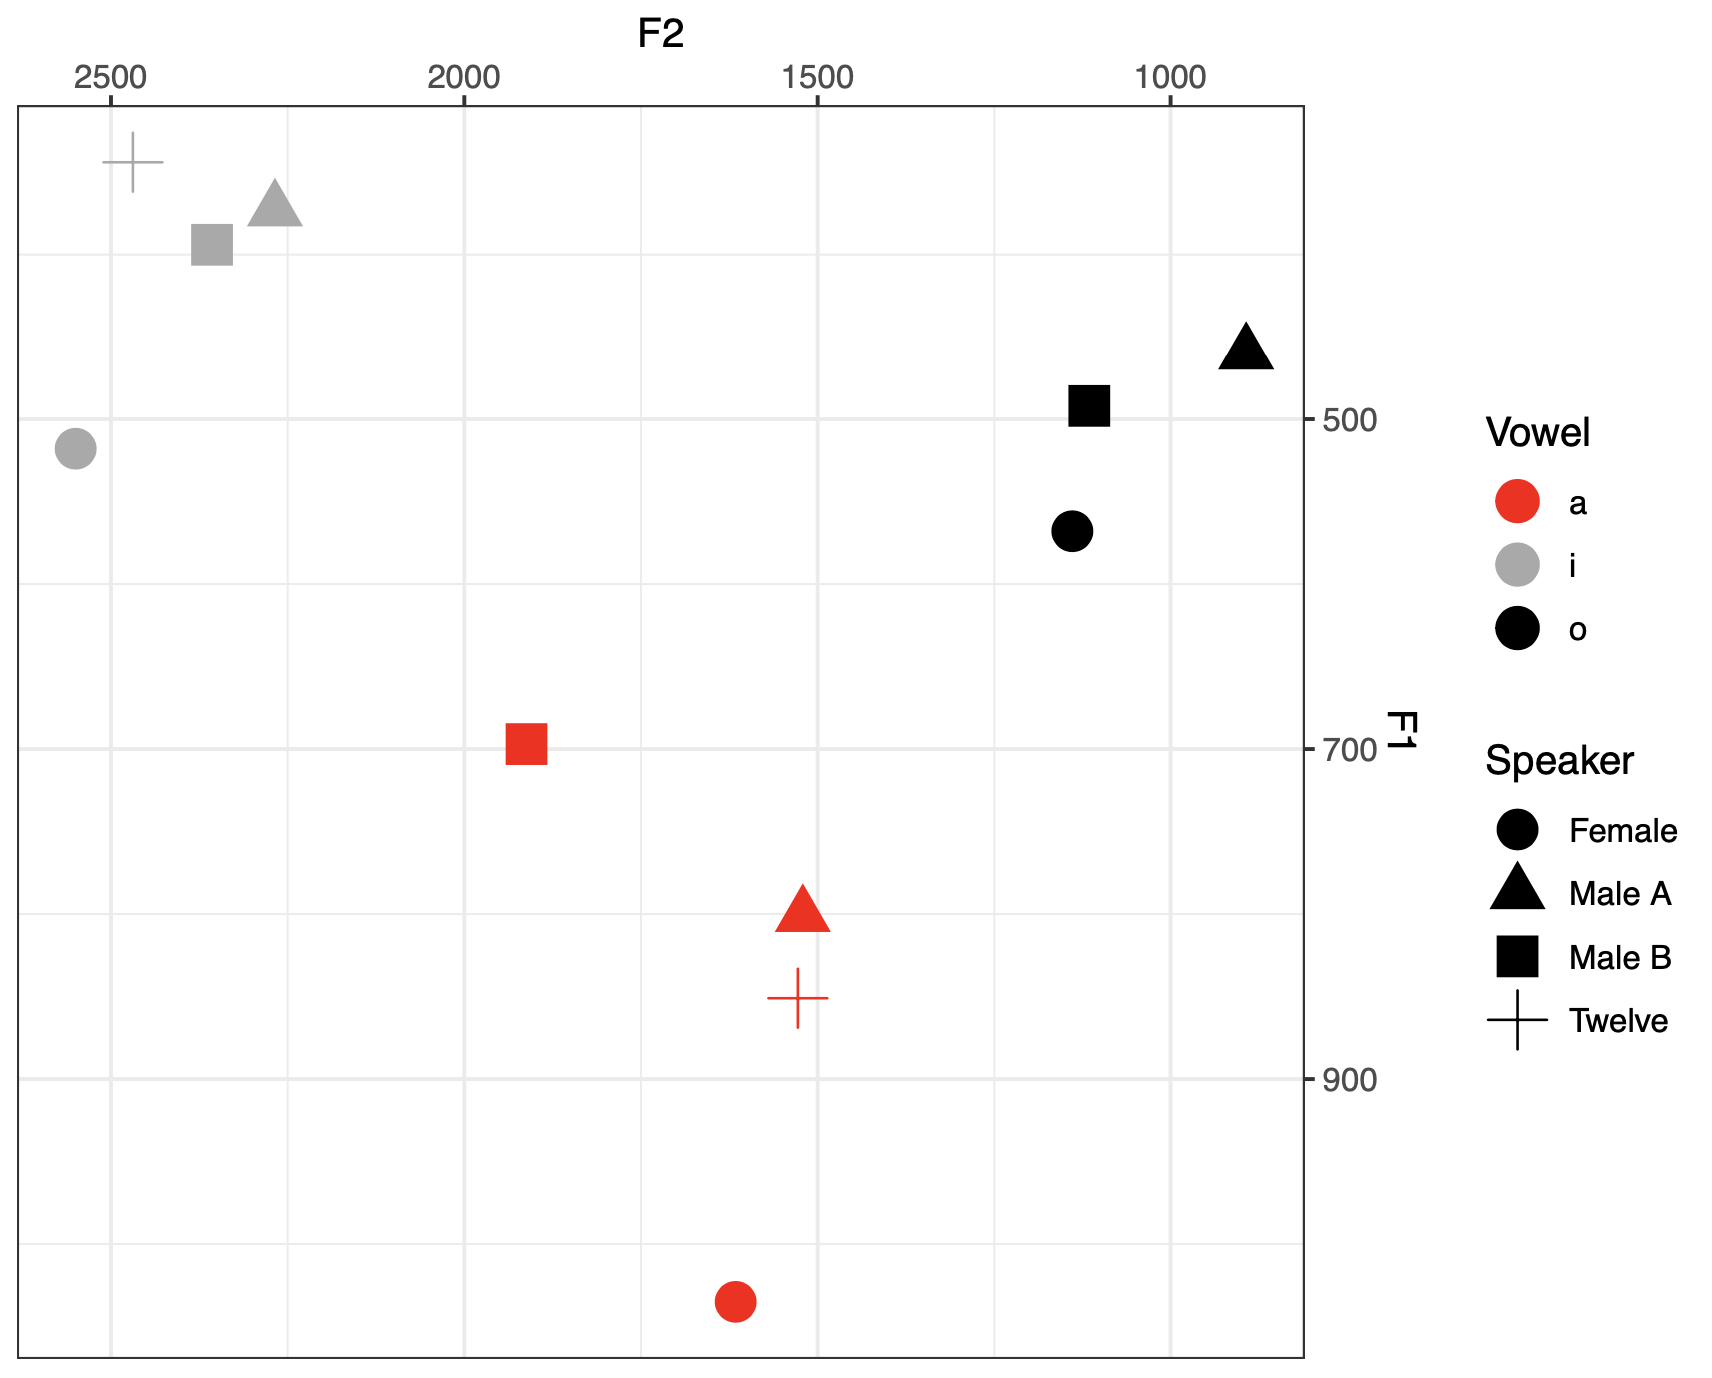
\includegraphics[width=0.8\textwidth]{figures/everett_figure2.png}
\caption{\label{fig:Figure 2}Vowel spaces based on values in \citew{everett1998acoustic} and \citew{de2010vowel}. The values in \citew{everett1998acoustic} were based on twelve adult speakers. Their mean F1 and F2 values are depicted here.}
\end{figure}

    In short, the Pirahã vowel inventory is small and occupies expected regions of the vowel space. The Pirahã consonant inventory is also small and consists of phonemes that are common cross linguistically. While the consonant and vowel inventories are small, this small size does not imply straightforward simplicity in its sound system. As noted above, previous work has documented some unusual allophonic variation and stress patterns \citep{everett1984relevance, everett1986piraha}. Finally, while the Pirahã phoneme inventory is atypical in terms of its size, it is not a statistical outlier in this regard since no languages are technically outliers at the low end of the inventory-size spectrum. Next we turn to some characteristics of the sound system that are unambiguously outliers from a typological perspective, characteristics that hint at the unique challenges that those acquiring Pirahã must overcome.

\section{How the Pirahã sound system is a global outlier}

    While phoneme inventories tell us something about the sounds that are meaningfully contrastive in a language, they tell us nothing about the commonality of those sounds or about the way those sounds are typically distributed within words in a language. The frequency and distribution of sounds within a language can offer a bit more detail regarding the role that individual phonemes play in a language. Recent research examining the intra-linguistic distribution and frequency of sounds has uncovered a variety of findings related to, for instance, the functional load and informativity of sounds. (See, for instance, \citew{wedel2013functional} and \citew{priva2017informativity}.) Other work has examined the frequency of sounds to demonstrate that, across the world’s languages, the frequency of consonants within a language generally follows a power-law distribution not dissimilar from that evident in the frequency of word types in a corpus \citep{everett2018similar}.
    
    If we examine the one hundred and fifty words in the UCLA Phonetics Lab Archive, we can see that such patterns also hold in Pirahã. Some of the phonemes in the language are particularly frequent in the words. To describe such patterns quantitatively, I imported the 150 words into R as strings of IPA characters. While this is obviously a small data set, it is worth noting that these 150 words contain many basic semantic concepts that one would expect to be common in actual speech. Using R \citep{venables2003r}, I obtained the relative frequency of Pirahã phonemes across these 150 words, which contain a total of 982 phoneme tokens. In these words for basic semantic concepts, /i/ is the most common phoneme, with 267 tokens (27.2\%). The second-most common phoneme is /a/, with 223 tokens (22.7\%). The remaining sounds, in descending order of frequency, are /o/ (12.1\%), /{\textglotstop}/ (7.9\%), /g/ (6.9\%), /b/ (5.8\%), [s] (4.9\%), [h] (4.1\%), /p/ (4.0\%), /t/ (2.2\%), and /k/ (2.1\%). Note that I separated [s] and [h]. The motivation for this separation will be evident below. A couple of observations are worth making, based on this ordering of sounds according to token frequency. First, while the language does have a common set of oral voiceless stops, namely /p/, /t/, and /k/, these are not common in the words. In fact, the latter two phonemes appear to be the least common in the language. At the other end of the spectrum, the three vowels are quite common, with /i/ and /a/ combined representing about half of all the language’s phoneme tokens in the data considered. This point bears stressing: Roughly half the sounds of Pirahã, judging from the words in the UCLA Phonetics Lab Archive, are variants of the high-front and low-central vowels.

    We can use the data to get a sense of some of the common sound sequences in the language, particularly in word-initial and word-final positions. The three most-common word-initial sounds are /{\textglotstop}/ (31.3\% of words), /b/ (12.7\%), and /k/ (12\%). Most of the occurrences of the latter phoneme are in word-initial position. A more striking pattern surfaces word-finally: 86\% of the transcribed words end in some variant of the /i/ vowel. It is worth noting that most of the words in the data are nouns, so there may be some lexical bias here as nouns are more likely to end in /i/. (Keren Madora, personal communication.)

    Word-medially, the most common sequence of two phonemes is /ai/, which surfaces 77 times in CVV syllables in these words. Taking these points together, we might state that a typical-sounding word in the language could begin with /{\textglotstop}/, end in /i/, and have an /ai/ sequence. The spectrogram of one such word, {\textglotstop}áapahai (“bird arrow”) is depicted in Figure 3.

\begin{figure}
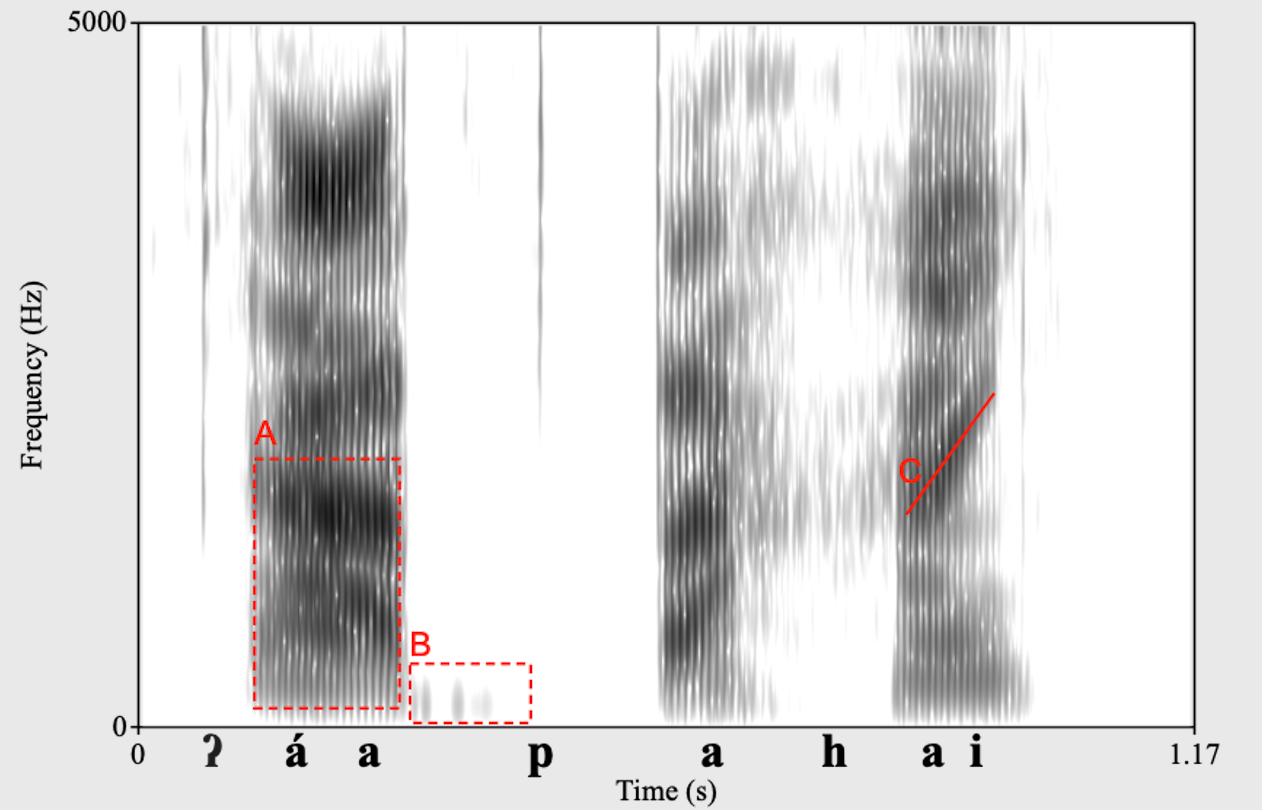
\includegraphics[width=\textwidth]{figures/everett_figure3.png}
\caption{\label{fig:Figure 3}Spectrogram of the word {\textglotstop}áapahai, “bird arrow” a typical word in Pirahã. The word is typical in that it only contains one oral consonant, is largely comprised of vowels and glottal consonants, begins with the glottal stop, and ends in /i/. Spectrogram created via PRAAT \citep{boersma2018praat}.}
\end{figure}

    In the highlighted features of the spectrogram in Figure 3, we can see the following: In A, the two /a/ vowels with distinct tones have very similar formant structures with respect to F1 and F2. This is evident in the dark bars within the rectangle. Yet the pitch is higher for the first /a/ vowel, which carries a high tone, as evidenced by the more compressed vertical striations that reflect vocal cord vibration. In B, we see that the /p/ consonant is relatively long and that the first half of it exhibits some voicing, though these characteristics may be partially an artifact of the deliberate pronunciation associated with word-elicitation tasks. Finally, C is a line highlighting the second formant in the /ai/ sequence, the most common sequence of two sounds in the language judging from these data. This rising F2 formant is found at the end of many of the words in the data set, as many end in /ai/.

    Given that the three most frequent phonemes in the language are /i/, /a/, and /o/, the ratio of Pirahã phoneme tokens that are vowels is quite high. In fact, there is evidence that the language relies on vowels more than any other language, at least judging from the Automated Similarity Judgement Program (ASJP) data \citep{wichmann2016asjp}. Each language variety in the ASJP data is represented by a transcribed word list for 40--100 basic concepts. In \citew{everett2017languages} I analyzed the transcriptions of the word lists in 4,012 language varieties, using the stringr packaged in R \citep{wickham2019package}. (The code is available in the SI of that study.) That analysis yielded a figure for each language variety, a figure representing the ratio of vowels as a proportion of all sounds in each word list. I referred to this ratio of vowels as a language’s “vowel index”. Unlike the phoneme inventory data evident in Figure 1, if a density distribution of all the “vowel indices” are plotted for the 4012 varieties, they approximate a Gaussian distribution \citep{everett2017languages}. 

    The goal of \citew{everett2017languages} was unrelated to Pirahã. Instead I aimed to test the hypothesis that very cold/dry air yields articulatory pressures against the usage of vowels in cold/dry regions. This hypothesis was based on extensive laryngology data suggesting that dry air increases jitter and perceived phonatory effort during speech. Since the publication of \citew{everett2017languages} more lab-based research has offered evidence of this, including work demonstrating effects in non-lab settings \citep{alves2019effect}. The results offered in \citew{everett2017languages} are correlational and could be coincidental though the pattern seems to be generally robust to the confounds of language relatedness and language contact. Furthermore, some researchers believe this distribution is due to ecological adaptivity owing to acoustic rather than articulatory factors \citep{maddieson2018language}. This line of inquiry is mentioned in the present context simply because it underscores an interesting feature of Pirahã, namely that it relies so heavily on vowels.


\begin{figure}
\centering
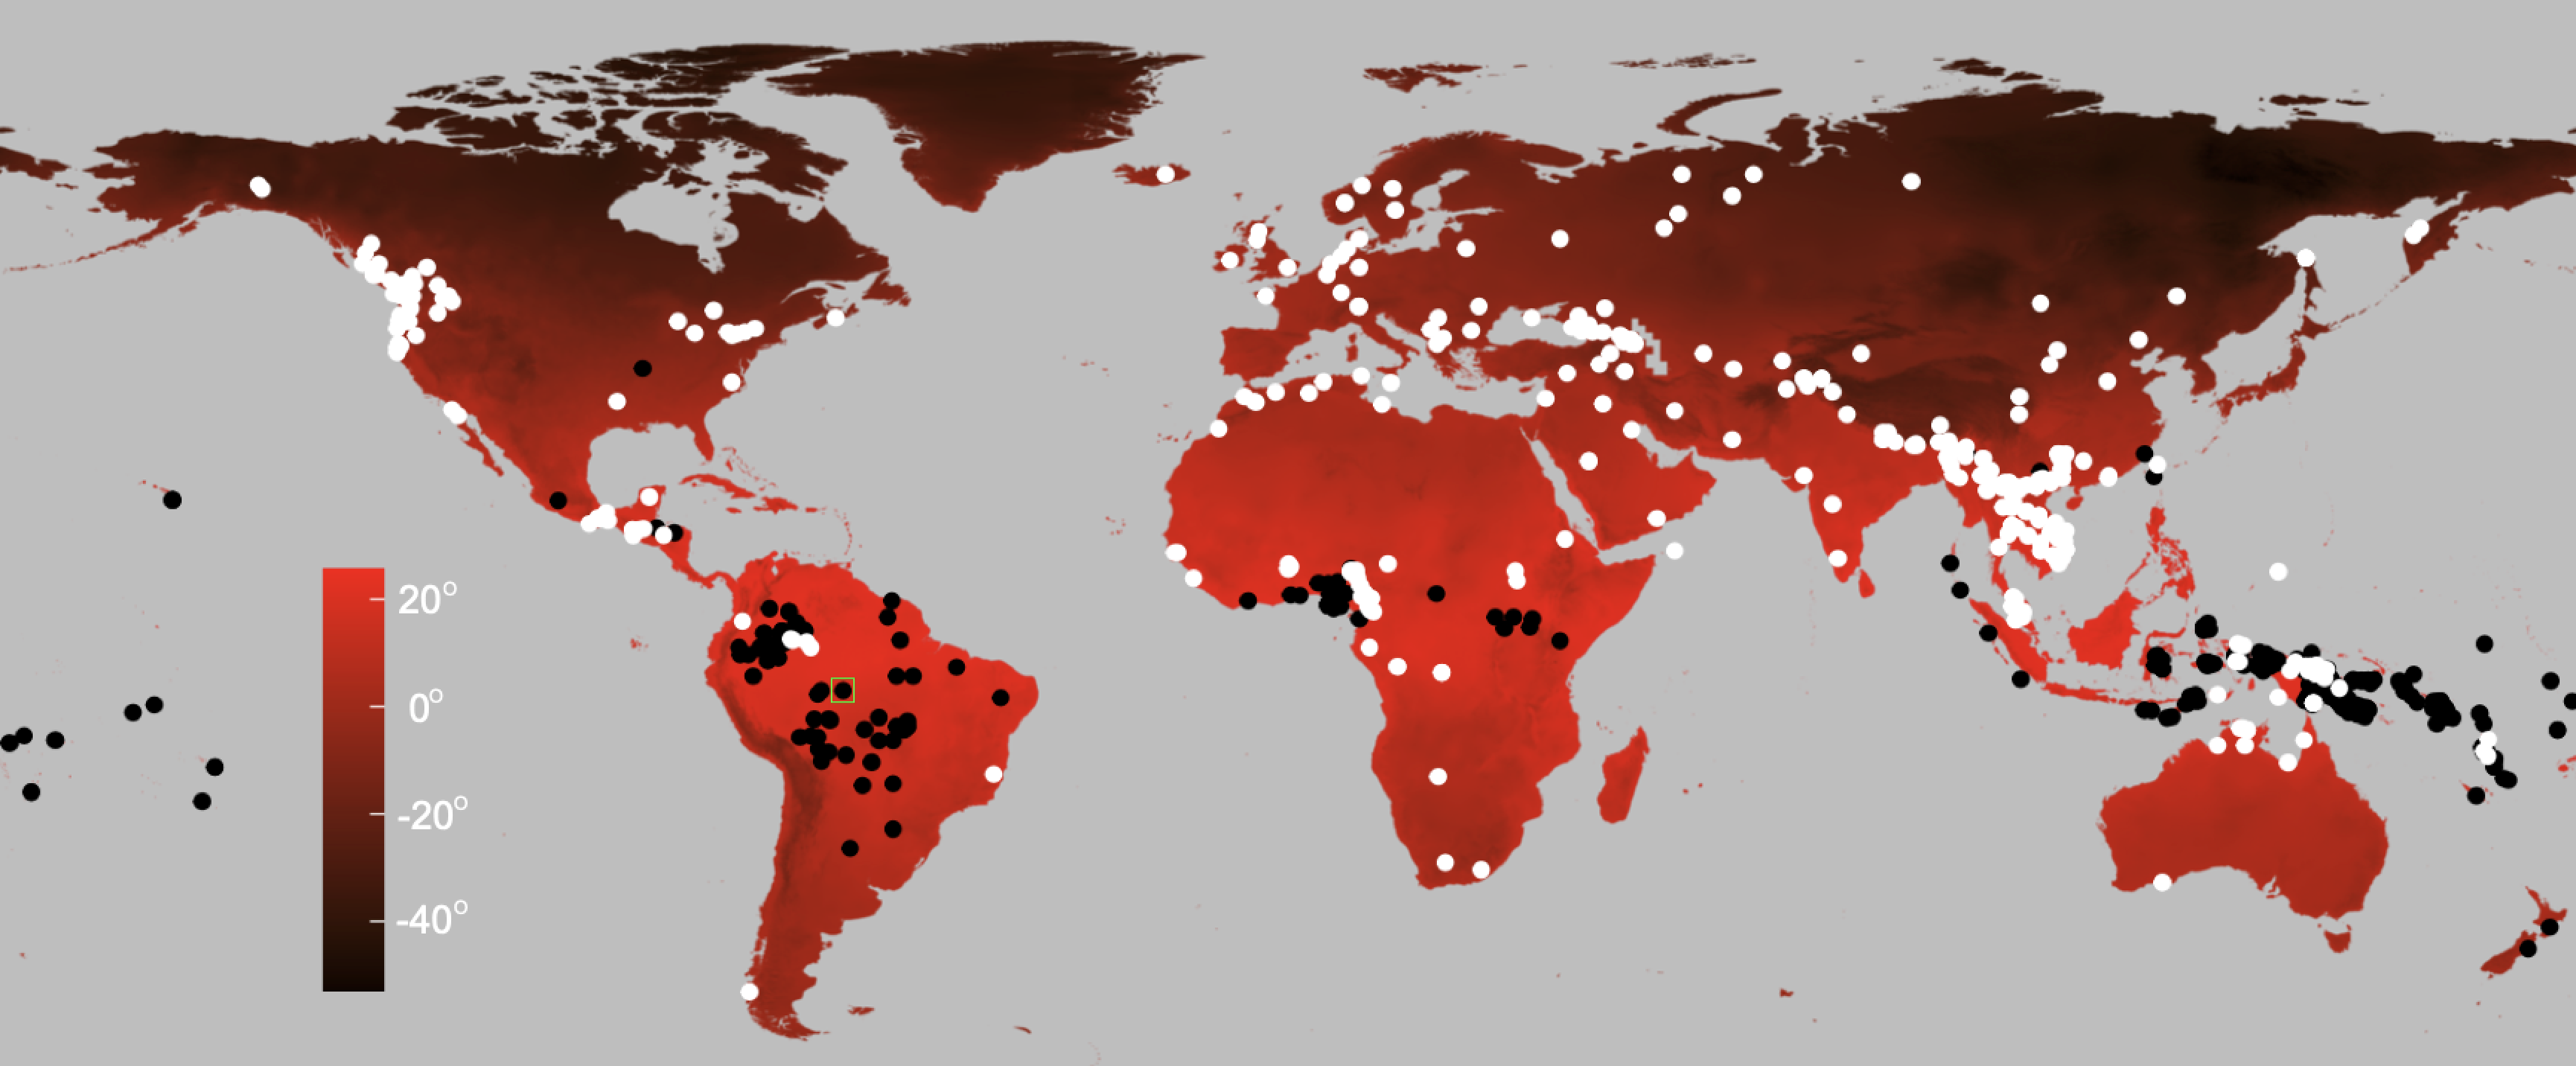
\includegraphics[width=1\textwidth]{figures/everett_figure4.png}
\caption{\label{fig:Figure 4}Four hundred language varieties from the ASJP database. The black dots represent the top 10\% of the 4012 language varieties in \citew{everett2017languages}, according to number of vowel sounds in a variety’s word list, as a ratio of all transcribed sounds in that list. The white dots represent the bottom 10\% of language varieties according to this metric. The map coloring is based on a raster layer created by the mean temperature of the coldest month, taken from the global bioclim data \citep{noce2020new}. Pirahã is highlighted with a square.}

\end{figure}

    Languages with the highest and lowest vowel “indices”, i.e. ratios of vowels-to-all-sounds in the ASJP word lists, are depicted in Figure 4. In the figure, Pirahã is highlighted with a square, as it is one of the languages with the top 10\% of vowel indices according to the ASJP data. As can be seen in Figure 4, Pirahã is typical in one sense: Nearly all of the languages with high vowel ratios occur in the tropics. In fact, only eight of the four hundred languages in the top 10\%, according to “vowel index”, are found above the Tropic of Cancer or below the Tropic of Capricorn. In contrast, 212 of the four hundred languages in the bottom 10\% occur outside the tropics. Setting aside the question of whether this is purely coincidental or due to some ecologically adaptive characteristics of languages, like those hypothesized by myself or Ian Maddieson, what is clear is that most languages that share this characteristic with Pirahã lie somewhere near the equator. It has long been known that many language families of the Pacific, Amazonia, and elsewhere rely heavily on simple syllable structures (and therefore rely heavily on vowels), yet the extent of the pattern evident in Figure 4 is surprisingly pronounced. Interestingly, Pirahã is an outlier even among Amazonian and South American languages in terms of its reliance on vowels. If we plot the vowel index data from \citew{everett2017languages} by continent, for instance, we see that the language would be an outlier on any continent according to this parameter. This is apparent in Figure 5.

\begin{figure}
\centering
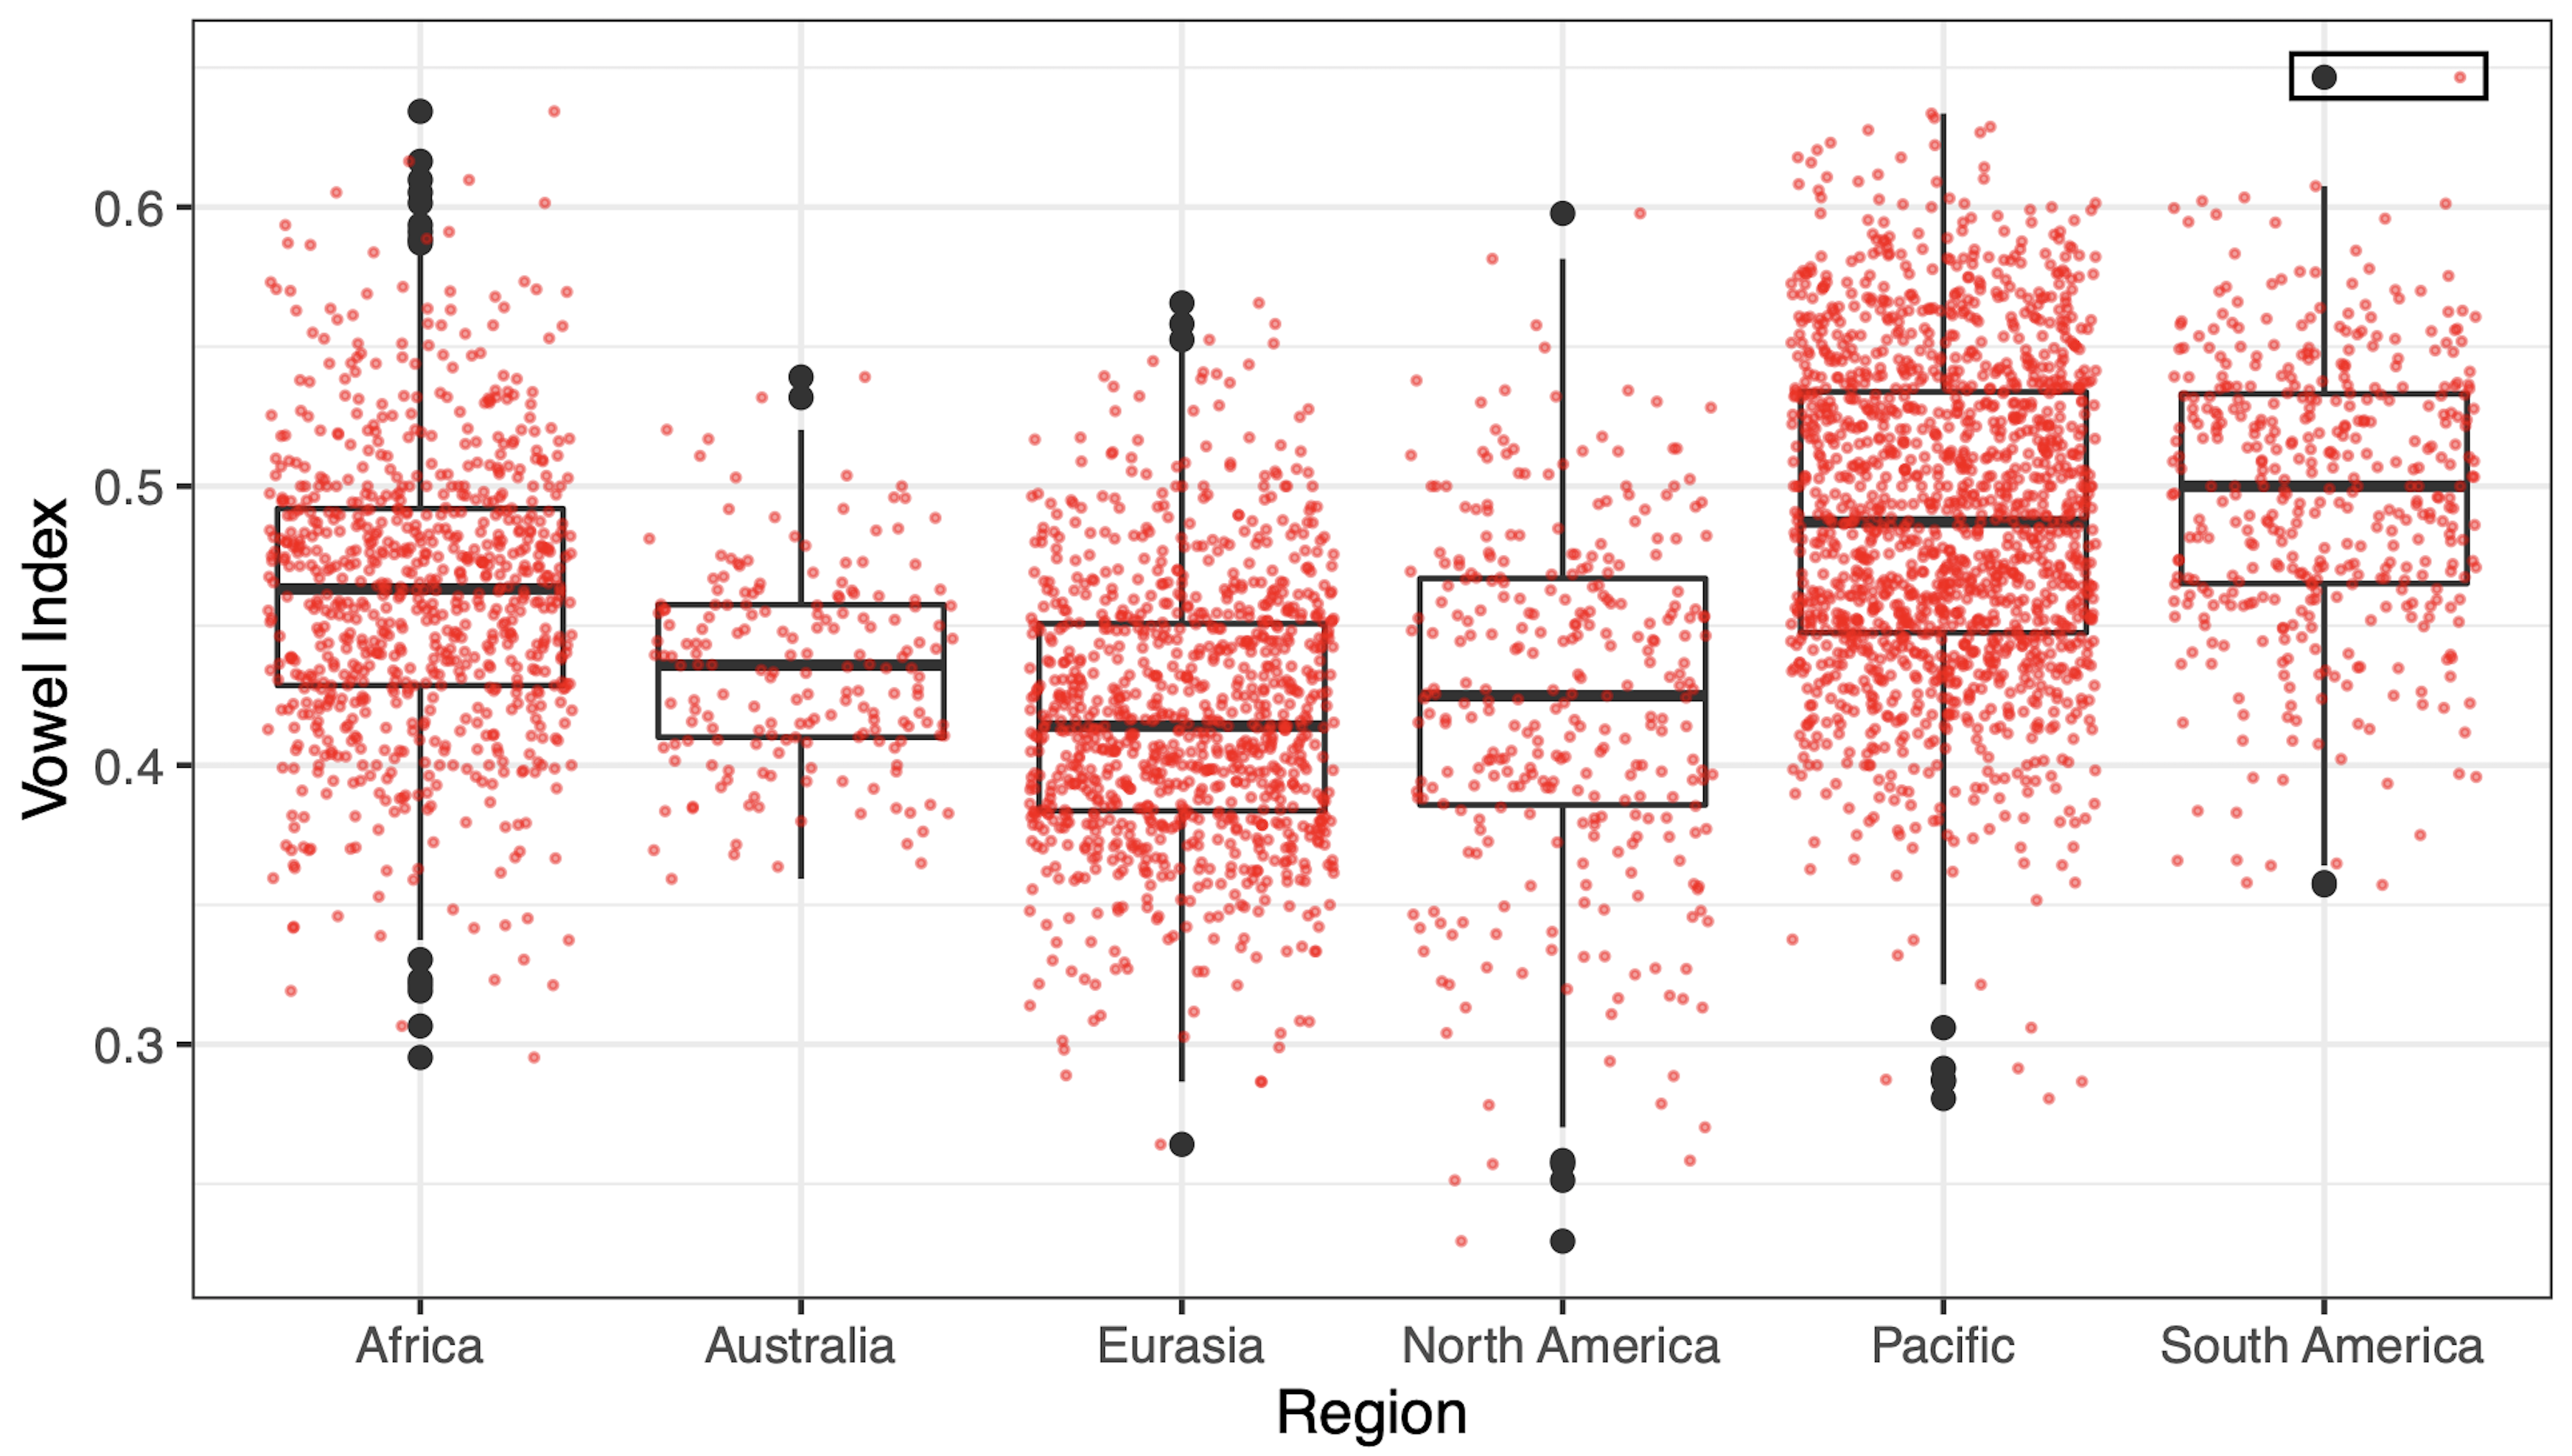
\includegraphics[width=1\textwidth]{figures/everett_figure5.png}
\caption{\label{fig:Figure 5}Contextualizing the high vowel reliance of Pirahã. “Vowel index” denotes the ratio of all transcribed sounds in an ASJP word list that are vowels. Each of 4012 language varieties is represented via a red dot. Dots are separated along the x-axis, within each column, via the jitter function in R. Pirahã is highlighted with a rectangle, which includes the black dot representing the outlier for the boxplot of South American languages in the data considered. All other regional outliers are also represented with black dots.}

\end{figure}

    One might wonder how representative the ASJP data are, given that they only encode 40--100 concepts per language variety and given that the transcription system used in the database is coarse. However, in those cases in which ASJP data are cross-referenced with other data, the results are generally quite similar. (see, e.g., \citew{everett2021speech}) We can test the data against the UCLA Phonetics Lab Archive data, for example. In the case of Pirahã, 609 of the 982 transcribed phoneme tokens in the UCLA data are vowels. In other words, 62\% of the sounds are vowels in that data set, in contrast to 64\% in the ASJP data. Even if we adopt the figure of 62\%, the language would remain an outlier in this respect. In the ASJP data, fewer than 1\% of the languages have “vowel indices” above 0.60.
    Even more remarkably, the language relies much less on consonants made with the lip or tongue, when contrasted to the world’s languages judging from the ASJP data. As noted above, the glottal consonant phonemes in the language are quite common. Taking the vowel frequency and glottal consonant frequency together, one might conclude that the load carried by laryngeal articulations is exceedingly high in the language. In the ASJP data 74\% of the transcribed Pirahã sounds are vowels or glottal consonants. In the 150 transcribed words in the UCLA Phonetics Lab Archive data, the exact same figure (74\%) obtains. (There is some modest overlap between the words in these data sets.) In other words, three quarters of all sounds in the basic Pirahã words in these data sets are not oral consonants. Using a function created via the stringr package in R (code available upon request), I calculated the ratio of sounds that are vowels or glottal consonants, across each of the same 4012 ASJP word lists in \citew{everett2017languages}. As evident in Figure 6, Pirahã is an even more pronounced outlier in this respect. Only eight of the 4012 language varieties have vowel-plus-glottal ratios greater than 70\%, and none obtain a figure as high as the 74\% in Pirahã.

\begin{figure}
\centering
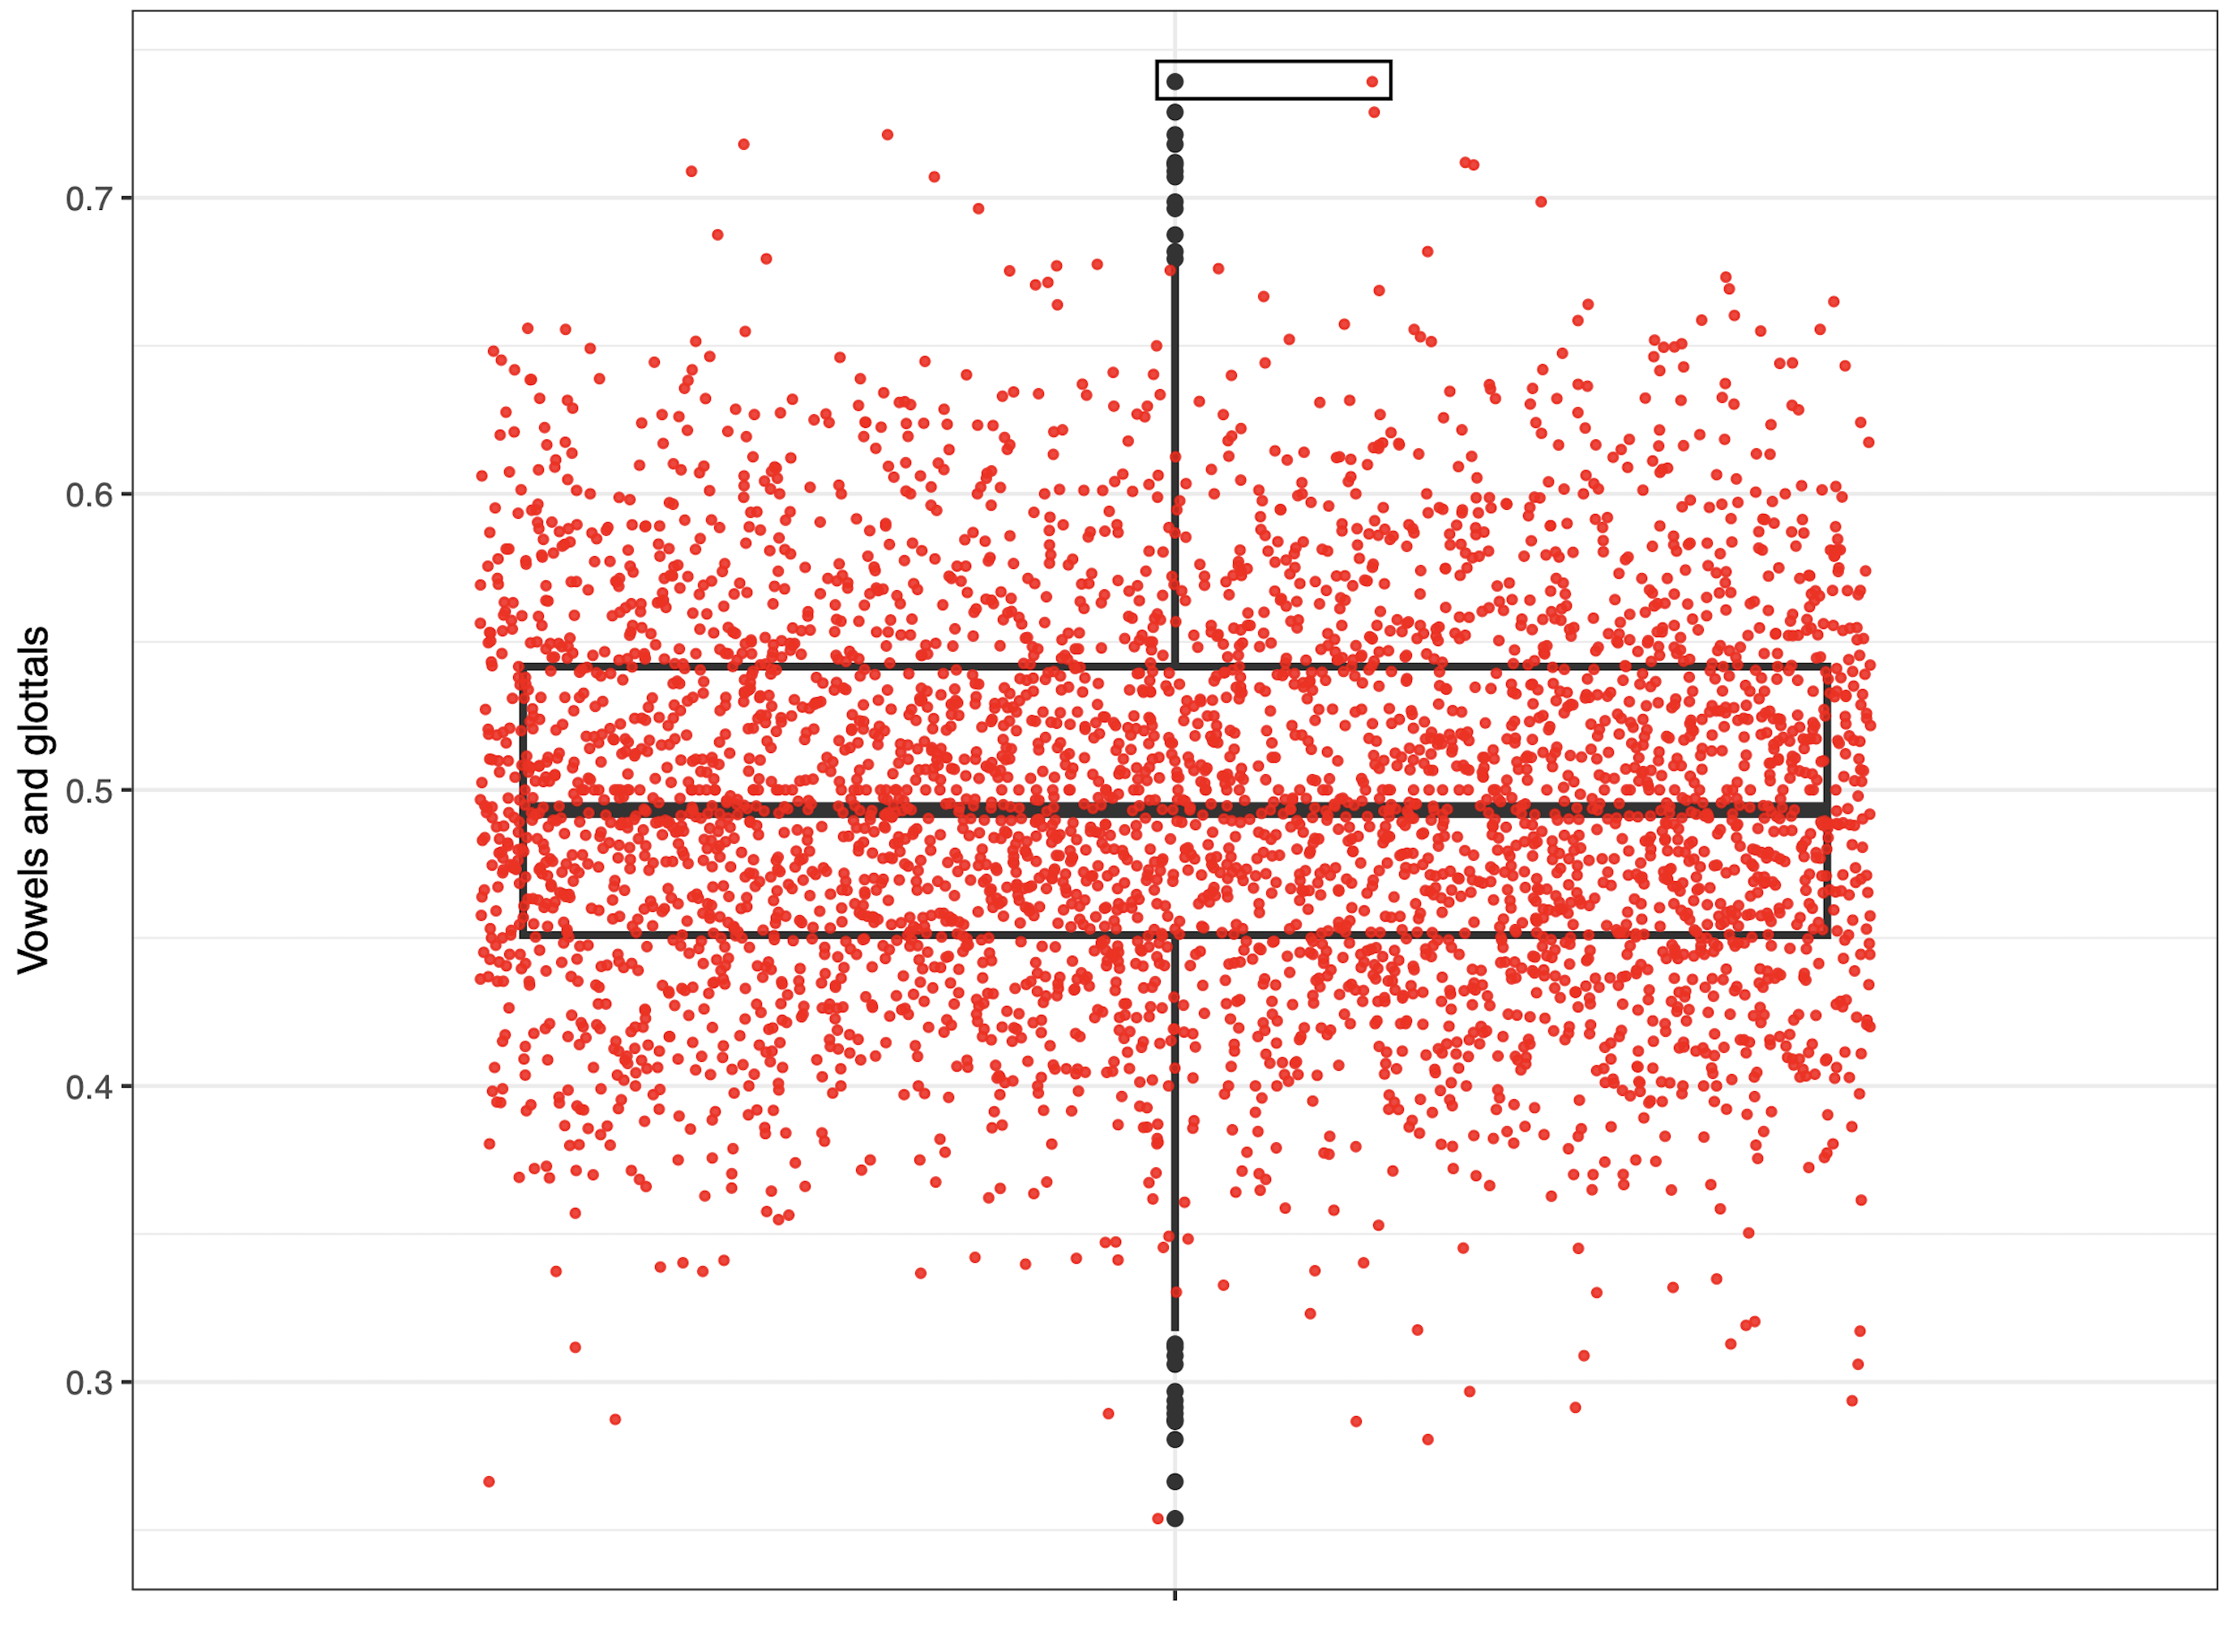
\includegraphics[width=1\textwidth]{figures/everett_figure6.png}
\caption{\label{fig:Figure 6}Ratio of sounds in ASJP word lists that are vowels or glottal consonants. Pirahã is highlighted via the rectangle. Dots are separated along the x-axis via the jitter function in R. 
}

\end{figure}

\section{Discussion and conclusion}

    Subsequent to the publication of my father’s 2005 paper in Current Anthropology \citep{everett2005cultural}, a number of papers were published contesting his claims. Oddly to some, these papers were published by scholars who had either no first-hand familiarity with the language, or had only marginal experience with the language, and certainly had no attested fluency in the language. Arguably, part of the explanation for the lack of successful follow-up research on Pirahã grammar, despite the extensive attention the debate surrounding it received, is that the language is so difficult to learn. There are, as of yet, no truly bilingual Pirahã who could serve as language resources to outsiders who do not speak the language. In my own experience with the people since I first spent some of my childhood in Pirahã villages some decades ago, I have seen numerous missionaries and linguists journey to the Pirahã, with varied aims. Some of these visitors have produced manuscripts on a variety of topics. Despite such work I have never seen an outsider maintain an extensive conversation in Pirahã, besides Dan Everett and Keren Madora. To my knowledge, no outsider has been able to demonstrate any degree of fluency. This is not meant as a criticism to those who have tried, instead I think this point merely underscores how difficult it is to learn the language. It took many years of work as missionaries, living in the village much of that time, before my parents could speak the language. I was there for much of this time, and can personally attest to the frustrations they conveyed and obstacles they overcame along the way in learning the language. Setting aside potential factors like appropriate training and aptitude, it seems unlikely that others could learn the language well without spending years on the effort. One would imagine that few interested parties would have the combination of time and funding that my parents dedicated to this task.
    
    This begs the question as to why the language is so difficult to acquire, apparently even when contrasted to some other Amazonian languages that FUNAI officials, missionaries, and others have acquired with high degrees of fluency. It is not just that it is difficult to gain fluency with the grammar of the language, many outsiders struggle stringing together basic words into simple phrases. I suspect that part of the reason may be Pirahã’s unusual phonetic and phonological characteristics that yield difficulty of both production and discrimination for outsiders. I have heard plenty of anecdotes from people visiting Pirahã villages suggesting that, for instance, the language sounds like “bees buzzing” and that it is hard to distinguish words given the heavy reliance on tones. Such stories hint at the key pattern outlined in Section 3 above: The language really is an outlier when it comes to its heavy reliance on vowels and glottal consonants or, framed differently, its limited reliance on oral consonants. Distinguishing a series of vowels, often with distinctive tones and relatively few intervening consonants, many of which are glottal, is an exceedingly difficult task for outsiders. Conversely, on the articulatory side, the language relies an inordinate amount on laryngeal gestures, including the creation of precise tone sequences without intervening oral consonants. This is an entirely unfamiliar enterprise to many. (Impressionistically, I also find it to be a difficult language to pronounce, despite my childhood experiences in Pirahã villages, even when contrasted to some other languages in the region.) Evidence now suggests that some languages are in fact more difficult to acquire, including by children, because of the unique characteristics of their sound systems. For instance, Danish, with so many vowel qualities, poses unique challenges for language acquisition for first and second-language learners \citep{trecca2021danish}. While Danish occupies the other end of the vowel-phoneme spectrum as Pirahã, in that it has many vowel phonemes, Pirahã relies more heavily on vowels than any other language according to the data discussed above. Further, there are interesting intervocalic differences in such sequences due to tone variations, and such sequences of tone-varying vowels appear to contribute to the challenge of acquisition by outsiders.
    
    Languages are profoundly diverse. An increasing number of scholars believe that this diversity
    is the chief explanandum that should occupy language researchers \citep{evans2009myth}. My father’s work on Pirahã underscored to many just how diverse languages could be. While debate will likely persist regarding some of his specific claims, perhaps especially because of the lack of other linguists who actually speak the language, it is clear to many of us that Pirahã exhibits some typological rarities that pose difficulties of various sorts to universalist approaches to language. That may say less about the language, of course, and more about the inadequacy of such approaches in the face of seemingly limitless linguistic variation. (As noted by \crossrefchaptert{16_piantadosi}, the influence of Chomskyan approaches to language appears to be crumbling, for reasons he elegantly lays out.) 
    
    In this paper I have outlined a few aspects of the sound system of Pirahã, suggesting that it is unique in some respects that are quantifiable. While the language is known to have a small phoneme inventory, I have suggested that this is arguably not the most remarkable feature of its sound system, partially because the global distribution of phoneme inventory is compressed in the manner evident in Figure 1. No known languages are technically outliers in terms of having small phoneme inventories, though some like Pirahã and Rotokas have unusually small inventories.  The phoneme inventory of Pirahã is small and consists of phonemes that are quite common crosslinguistically. This may give the impression of simplicity of the language’s sound system, but I have suggested this would be inaccurate. Instead, I have argued that perhaps the most remarkable feature of the Pirahã sound system is its extreme reliance on vowels, and also its combined reliance on vowels and glottal consonants, judging from analyses of the ASJP data and the UCLA Phonetics Lab Archive data. It is a regional and global outlier in both of these respects. As a result, the language is characterized by strings of vowels with varying tones and limited intervening oral consonants, a fact that presents perceptually and articulatory unique characteristics that likely contributes to its difficulty of acquisition for outsiders. If someone spends time listening to and producing Pirahã, they are unlikely to be left with an impression that the sound patterns in the language are simple. Quite the contrary, in my experience they may be baffled by its sound patterns, potentially because of the language’s status as a typological outlier in the sense that I have outlined here.

\printbibliography[heading=subbibliography,notkeyword=this]

\end{document}
